\begin{frame}{3.6 좌굴방지가새}

\textbf{3.6.1 일반사항}

이 절은 강재코어와 강재코어의 좌굴을 구속하는 좌굴방지 시스템으로 구성되는 좌굴방지가새에 적용한다. 

\textbf{3.6.2 좌굴방지가새의 강성}

3.6.2.1 선형동적절차

\begin{enumerate}
	\item[(1)] 좌굴방지가새 부재의 탄성구간 강성은 좌굴이 구속된 항복코어요소와 전이요소가 직렬로 연결된 것으로 산정하며, 이 때 전이요소는 구속된 항복코어요소의 단부와 거셋플레이트의 접합부의 역학적 특성이 포함되어야 한다. 
	\item[(2)] 거셋플레이트와 보--기둥 접합부는 가새의 축강성에 대해 상대적으로 강접으로 가정할 수 있다. 
\end{enumerate}

\end{frame}



\begin{frame}{3.6 좌굴방지가새}

	\textbf{3.6.2 좌굴방지가새의 강성}

	3.6.2.2 비선형정적절차
	
	\begin{enumerate}
		\item[(1)] 좌굴방지가새 부재의 탄성구간 강성은 3.6.2.1에 따라 산정한다. 
		\item[(2)] 좌굴방지가새 부재의 비선형 부재력--변형 모델링은 실험이나 정밀해석을 통해 얻어진 관계를 사용하거나, 그림 1-1과 같은 일반화된 부재력--변형 관계로부터 다음을 따른다. 
		\begin{enumerate}[label=\large\protect\textcircled{\small\arabic*}]
			\item $\Delta_y$는 3.6.3.2절에 정의된 가새의 예상항복강도에 상응하는 축변형으로 그림 3-1 곡선 $B$점에서의 강도 및 변형이다. 
			\item 기타 모델링 변수는 표 3-7 및 3.5.3.3절을 따른다. 
			\item 표 3-7의 모델링변수 $b$ 이후의 최대강도 이후 기울기는 잔류강도가 거의 0에 가까울 때까지 음의 항복강성을 사용할 수 있다. 
		\end{enumerate}	
	\end{enumerate}
\end{frame}



\begin{frame}{3.6 좌굴방지가새}

	\textbf{3.6.2 좌굴방지가새의 강성}

	3.6.2.3 비선형동적절차
	
	좌굴방지가새 부재의 이력거동 모델링은 실험이나 정밀해석을 통해 얻어진 관계를 사용할 수 있으며, 포락곡선으로는 3.5.2.2절의 일반화된 하중--변형관계를 해석에 사용할 수 있다.  
\end{frame}	





\begin{frame}{3.6 좌굴방지가새}

	\textbf{3.6.3 좌굴방지가새의 강도}

3.6.3.1 일반사항

강재코어로부터 발현될 수 있는 최대강도 산정 시 재료의 변형도경화 효과와 인장강도에 대한 압축 초과강도를 고려한 조정값을 포함시켜야 한다. 

3.6.3.2 선형동적절차

\begin{enumerate}
	\item[(1)] 좌굴방지가새의 예상부재강도 $Q_{CE}$는 코어의 순단면적과 예상재료강도 $F_{ye}$의 곱으로 산정한다. 
	\item[(2)] 강도산정 및 모델링을 위한 예상재료강도 $F_{ye}$는 설계기준항복응력과 본 가이드의 2장에 정의된 $R_y$의 곱으로 산정하며, 예상재료강도 $F_{ye}$가 시험에 의해 결정된 경우에는 $R_y$를 적용하지 않는다. 
	\item[(3)] 강재코어로부터 압축에 의해 전달되는 최대 하중은 $\beta\omega Q_{CE}$ 식으로 산정하고, 인장에 의해 전달되는 최대 하중은 $\omega Q_{CE}$ 식으로 산정하며 아래의 사항을 따른다. 
	\begin{enumerate}[label=\large\protect\textcircled{\small\arabic*}]
		\item $\beta$와 $\omega$는 각각 압축강도조정계수와 변형도경화조정계수로 $\ulcorner$건축물 강구조 설계기준$\lrcorner$의 4.19절에 정의된 품질보증 시험에 기초한다.
		\item 선형동적절차에 대해 시험을 통한 규정이 되지 않은 경우 계수 $\beta$와 $\omega$의 값은 각각 1.1과 1.3을 사용할 수 있다.
	\end{enumerate}
	\end{enumerate}
	\end{frame}
	
\begin{frame}{3.6 좌굴방지가새}

	\textbf{3.6.3 좌굴방지가새의 강도}	

3.6.3.2 선형동적절차
	\begin{enumerate}		
	\item[(4)] 항복강도가 일정한 범위로 규정된 경우, 최대가새강도를 결정하기 위한 예상재료강도 $F_{ye}$는 범위 내 최대인장응력을 사용한다.
	\item[(5)] 가새 접합부의 하한부재강도 $Q_{CL}$는 $\ulcorner$건축물 강구조 설계기준$\lrcorner$에 따라 산정하며, 재료강도는 하한항복강도 $F_{yLB}$를 사용한다. 
	\end{enumerate}
\end{frame}	


\begin{frame}{3.6 좌굴방지가새}

	\textbf{3.6.3 좌굴방지가새의 강도}

	3.6.3.6 비선형정적 및 동적절차
	
	\begin{enumerate}
		\item[(1)] 비선형정적절차의 경우 표 3-1에 따라 그림 1-1과 같은 비선형 부재력--변형 관계를 결정한다. 좌굴방지가새의 예상부재강도 $Q_{CE}$는 선형절차와 동일한 값을 사용한다. 
	\begin{enumerate}[label=\large\protect\textcircled{\small\arabic*}]
		\item 그림 9-2의 $C$점은 인장에 대해서는 $\omega Q_{CE}$이고 압축에 대해서는 $\beta \omega Q_{CE}$이다. 
		\item 압축강도 산정을 위한 압축강도조정계수 $\beta$ 및 변형도경화조정계수 $\omega$는 9.5.4.3.2절 및 $\ulcorner$건축물 강구조 설계기준$\lrcorner$을 따른다. 
	\end{enumerate}		
		\item[(2)] 비선형동적절차의 이력거동 모델링은 실험이나 정밀해석을 통해 얻어진 관계를 사용할 수 있으며, 포락곡선으로는 3.5.3.3절에 사용된 모델을 적용할 수 있다. 
	\end{enumerate}
\end{frame}	


	\begin{frame}{3.6 좌굴방지가새}

	\textbf{3.6.4 좌굴방지가새의 허용기준}

	3.6.4.1 일반사항

	\begin{enumerate}
		\item[(1)] 인장이나 압축을 받는 가새 부재는 변형지배거동으로 분류한다. 
		\item[(2)] 거셋플레이트, 볼트, 용접 및 기타 접합요소를 포함한 가새접합부에 작용하는 압축, 인장, 전단 및 휨은 힘지배거동으로 분류한다. 
		\item[(3)] 유사한 접합상세에 대하여 실험으로 거동이 규명된 경우 거셋플레이트는 변형이 지배하는 것으로 고려할 수 있다. 
	\end{enumerate}
	
	3.6.4.2 선형동적절차
	
	\begin{enumerate}
		\item[(1)] 강재요소의 $m$계수는 표 3-8을 따른다. 
		\item[(2)] 표 3-1의 $m$계수는 $\ulcorner$건축물 강구조 설계기준$\lrcorner$의 절차에 따른 실험결과가 제출된 경우에만 허용된다. 
		\item[(3)] $\ulcorner$건축물 강구조 설계기준$\lrcorner$의 변형항목 $\Delta_{bm}$은 BSE-1E 위험도에서 최대 100\% 또는 BSE-2E나 BSE-2N 위험도에서 최대 65\%까지 허용된다. 
	\end{enumerate}

	\end{frame}
	
	
	\begin{frame}
	\begin{figure}
		\centering
		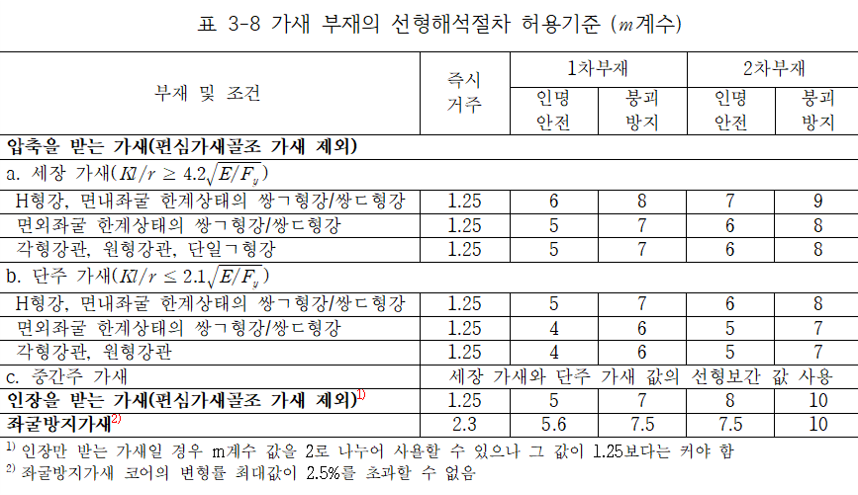
\includegraphics[width=.99\textwidth]{table3-8}
	\end{figure}
\end{frame}	
	
	
	
	
	\begin{frame}{3.6 좌굴방지가새}

	\textbf{3.6.4 좌굴방지가새의 허용기준}
	
3.6.4.3 비선형 정적 및 동적절차	

	\begin{enumerate}
		\item[(1)] 요소의 변형한계는 표 3-2, 3-6 및 3-7의 값을 사용한다.  
		\item[(2)] 표 3-7의 허용기준 및 모델링 변수는 $\ulcorner$건축물 강구조 설계기준$\lrcorner$의 절차에 따른 실험결과가 제출된 경우에만 허용된다. 
		\item[(3)] $\ulcorner$건축물 강구조 설계기준$\lrcorner$의 변형항목 $\Delta_{bm}$은 BSE-1E 위험도에서 최대 100\% 또는 BSE-2E나 BSE-2N 위험도에서 최대 65\%까지 허용된다. 
	\end{enumerate}
	\end{frame}	



\begin{frame}
	\begin{figure}
		\centering
		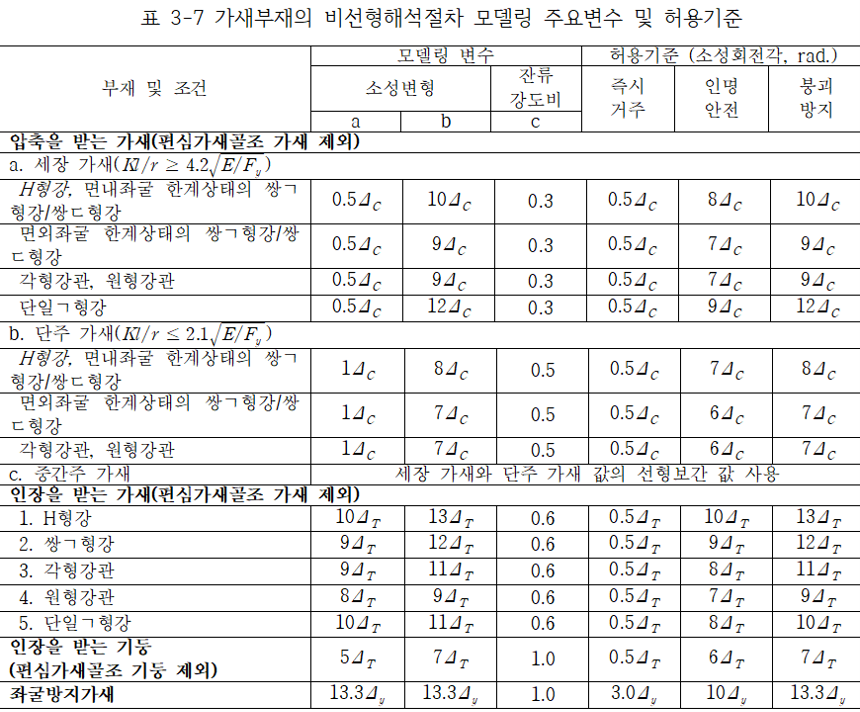
\includegraphics[width=.99\textwidth]{table3-7}
	\end{figure}
\end{frame}	
